\documentclass[11pt]{article}

\usepackage[margin=1.1in]{geometry}
\usepackage{amsmath,amssymb,amsthm}
\usepackage{graphicx}
\usepackage{booktabs}
\usepackage{microtype}
\usepackage[round]{natbib}
\usepackage{xcolor}
\usepackage[colorlinks=true,linkcolor=blue!50!black,citecolor=blue!50!black,urlcolor=blue!50!black]{hyperref}

\graphicspath{{figures/}}
% generated by toy_path.py -- do not edit
\newcommand{\pathSeed}{0}
\newcommand{\pathN}{10}
\newcommand{\pathSubsets}{1024}
\newcommand{\pathIntervals}{56}
\newcommand{\pathBothConn}{20}
\newcommand{\pathFreeSet}{\{0,1,2,3,4,6\}}
\newcommand{\pathFreeGa}{73.88}
\newcommand{\pathFreeGb}{58.52}
\newcommand{\pathFreeProd}{4323.7}
\newcommand{\pathIvSet}{\{0,1,2,3,4,5\}}
\newcommand{\pathIvGa}{70.10}
\newcommand{\pathIvGb}{61.59}
\newcommand{\pathIvProd}{4317.6}
\newcommand{\pathIvCostPct}{0.14}
\newcommand{\pathBothSet}{\{0,1,2,3,4,5\}}
\newcommand{\pathBothProd}{4317.6}
\newcommand{\pathBothCostPct}{0.14}
% generated by toy_grid.py -- do not edit
\newcommand{\gridSeed}{0}
\newcommand{\gridN}{16}
\newcommand{\gridSubsets}{65536}
\newcommand{\gridFeasible}{1256}
\newcommand{\gridFreeProd}{2239.3}
\newcommand{\gridFreePieces}{2}
\newcommand{\gridFreeASet}{\{0,1,2,4,7,11,14,15\}}
\newcommand{\gridContProd}{2053.9}
\newcommand{\gridContASet}{\{0,1,4,8,11,12,13,14,15\}}
\newcommand{\gridCostPct}{8.28}
\newcommand{\gridPieceP}{\{0,1,2,4\}}
\newcommand{\gridCutU}{0}
\newcommand{\gridCutV}{15}
\newcommand{\gridCutC}{\{3,5,6,8\}}
\newcommand{\gridCutLhsFree}{0}
\newcommand{\gridCutRhsFree}{1}


\newtheorem{prop}{Proposition}
\newtheorem{obs}{Observation}
\theoremstyle{definition}
\newtheorem{example}{Example}

\newcommand{\ga}{g_a}
\newcommand{\gb}{g_b}
\newcommand{\ua}{u_a}
\newcommand{\ub}{u_b}

\title{Contiguous Nash territory division:\\ the mathematical setup and the single-tree solver}
\author{Territory-division project\thanks{A self-contained companion to
\texttt{nash\_territory\_division.tex} and the contiguity development programme
(\texttt{research/contiguity/}). Solver numbers are from the harness runs of
2026-08-29/30 (\texttt{research/contiguity/RESULTS.md}); every number in the toy
examples is computed by \texttt{toy\_path.py} / \texttt{toy\_grid.py} and injected
as a macro, never transcribed.}}
\date{2026-08-30}

\begin{document}
\maketitle

\begin{abstract}
\noindent
Two merging sales forces must divide a set of postal territories (ZCTAs) between the two
legacy representatives who overlap on each region. We state the model --- maximum Nash
welfare over indivisible zips at a zero disagreement point, with hard geographic
contiguity --- and develop the geometry that makes its computational behaviour
intelligible: the feasible set is a finite point cloud in gain space, the free optimum is
a hyperbola tangency, contiguity thins the cloud, and the solver's job is to prove that
nothing above a hyperbola survives the thinning. We describe the two families of cutting
planes (outer-approximation tangents for the concavified objective, root-free separator
cuts for contiguity), why their convergence theories multiply in a multi-tree loop and
compose in a single branch-and-cut tree, and the leading implementation,
\texttt{scip\_tree}. Two fully enumerable toy instances --- ten zips on a path,
sixteen on a grid --- reproduce every phenomenon at a size where it can be drawn.
\end{abstract}

\section{The problem}\label{sec:problem}

For each postal code (zip) $z$ in a contested region there are three nonnegative numbers:
firm-A sales $A_z$, firm-B sales $B_z$, and the market opportunity $M_z$. Two parameters
translate them into what a territory is worth to each representative: the
\emph{transfer capture} $\theta\in[0,1]$, the fraction of the other rep's book an
inheriting rep retains, and the \emph{headroom credit} $\lambda\in[0,1]$, the rate at
which untapped opportunity counts against booked production. With
$c_1=1-\lambda$ and $c_2=\theta(1-\lambda)$ (the \emph{net} headroom convention),
\begin{equation}\label{eq:utils}
\ua(z) \;=\; c_1 A_z + c_2 B_z + \lambda M_z,
\qquad
\ub(z) \;=\; c_2 A_z + c_1 B_z + \lambda M_z ,
\end{equation}
and the model requires pointwise nonnegative headroom,
$M_z \ge \max(A_z+\theta B_z,\; B_z+\theta A_z)$. The reference values used throughout
are $\theta=0.40$, $\lambda=0.30$.

An \emph{allocation} is a subset $S\subseteq Z$ of the region's zips, read as ``rep $a$
gets $S$, rep $b$ gets $Z\setminus S$.'' Utilities are additive, so each side's
\emph{gain} is a bundle utility:
\begin{equation}\label{eq:gains}
\ga(S)=\sum_{z\in S}\ua(z), \qquad \gb(S)=\sum_{z\notin S}\ub(z).
\end{equation}

\paragraph{The criterion.}
The allocation is chosen to maximise the Nash product,
\begin{equation}\label{eq:nash}
\max_{S\subseteq Z}\;\; \ga(S)\cdot \gb(S),
\end{equation}
i.e.\ \emph{maximum Nash welfare} (MNW) --- the Nash bargaining solution
\citep{nash1950} at disagreement point $d=(0,0)$. The zero disagreement point is a
modelling decision with three grounds, in descending force. First, the threat point is
not available: after the merger neither rep can revert to a legacy book, so the payoff
to failed bargaining is zero, not the status quo ante. Second, at a zero baseline MNW
over indivisible goods is Pareto efficient and envy-free up to one good (EF1) as a
theorem \citep{caragiannis2019}; subtracting constants from the utilities voids the
guarantee. Third, it restores the correspondence with continuum Nash bargaining, whose
solution at $d=0$ is an optimal-transport map \citep{warren2025}. It also removes a
failure mode outright: gains \eqref{eq:gains} are positive by construction, so the
bargaining set cannot be empty for any parameter values.

\paragraph{Census decomposition.}
Nationally there are many reps per firm. The \emph{census} intersects the two legacy rep
maps and decomposes the country into bilateral components: each contested component is a
region $Z$ with one A-rep and one B-rep, and \eqref{eq:nash} is solved independently per
component. Production-size components run to 400--800 zips. (Dense many-on-many
components need a multi-agent extension --- component-level MNW $\sum_i \log g_i$ ---
outside this note's scope.)

\paragraph{Contiguity.}
The operational requirement that a rep's territory be drivable enters as a \emph{hard
constraint}: on the Rook-adjacency graph $G=(Z,E)$ of the region's zips, each side's
allocation must induce a connected subgraph. Precisely, since the pair graph itself may
have several connected components, the constraint is \emph{component-wise}: inside each
connected component $K$ of $G$, both $S\cap K$ and $K\setminus S$ must be connected in
$G[K]$ or empty. No compactness penalty appears in the objective ($\rho=0$ is the
model); a perimeter tie-break, when wanted, is a lexicographic post-pass, never a
penalty. Connected fair division is NP-hard already for two agents with identical
valuations \citep{deligkas2021}, so an exact method with certificates --- not a closed
form --- is the realistic target; see also \citet{bouveret2017,bilo2022} for the
fair-division-on-graphs setting and \citet{bei2022} for price-of-connectivity bounds
(none are known for Nash welfare).

\section{Geometry of the free problem}\label{sec:geometry}

Everything about \eqref{eq:nash} becomes visual in \emph{gain space}. Map every
allocation to the point $\big(\ga(S),\gb(S)\big)\in\mathbb{R}^2_{\ge0}$: the feasible
set is a finite cloud of $2^n$ points (generically fewer, by coincidences), contained in
the box $[0,G_a^{\max}]\times[0,G_b^{\max}]$ with $G_a^{\max}=\sum_z\ua(z)$,
$G_b^{\max}=\sum_z\ub(z)$. Moving one zip $z$ from $b$ to $a$ translates the point by
$(+\ua(z),-\ub(z))$: the cloud is the Minkowski-type sum of $n$ two-point sets, anchored
at $(0,G_b^{\max})$. Figure~\ref{fig:path} (left) shows the actual cloud of the
$n=\pathN$ path toy of Section~\ref{sec:toys}.

Three features of the picture do real work.

\begin{itemize}
\item \textbf{The Nash optimum is a hyperbola tangency.} Level sets of the objective are
hyperbolas $\ga\gb=\text{const}$; the optimum is the point of the cloud touching the
highest one. Because the level sets are strictly monotone, the optimum lies on the
cloud's Pareto frontier --- Pareto efficiency is by construction, and ``equalising''
criteria that minimise $|\ga-\gb|$ can leave the frontier entirely and hurt both sides
at once; Nash cannot.
\item \textbf{The frontier is near-linear, so weighted sums fail.} A scalarisation
$w\,\ga+(1-w)\,\gb$ picks the frontier point supported by a line of slope
$-w/(1-w)$. When the frontier hugs a line --- which additive utilities with many small
zips produce --- almost every $w$ selects a corner, and the interesting middle of the
frontier is invisible to the method. The hyperbola, curved against the frontier's
flatness, selects the interior point stably.
\item \textbf{The fractional relaxation is the ratio sort.} Allow fractional shares
$x_z\in[0,1]$. The relaxed feasible region in gain space is the zonotope spanned by the
segments $\{x_z\,(\ua(z),-\ub(z))\}$, whose upper boundary is traced by sorting zips by
the exchange rate $r_z=\ua(z)/\ub(z)$ and adding them in decreasing order. Maximising
$\ga\gb$ over that boundary is the discrete-optimal-transport relaxation of the problem,
and its value is an \emph{upper bound} on \eqref{eq:nash}. Rounding it --- take the best
prefix of the ratio order --- is the ``prefix heuristic.''
\end{itemize}

\paragraph{Why the prefix rule is not a theorem.}
The classical threshold argument is marginal: at an optimum, no zip's transfer should
help, and treating $\ga,\gb$ as fixed while $z$ moves gives a ratio threshold. But
discretely the gains jump by $\ua(z),\ub(z)$ --- finite amounts --- and the argument
only certifies a local optimum of the exchange neighbourhood, not of \eqref{eq:nash}.
Measured against exhaustive enumeration the best prefix is optimal only ${\sim}45\%$ of
the time at any size ($n=6$: optimal $40\%$, mean shortfall $3.91\%$, worst $53.9\%$;
$n=14$: $45\%$, $0.57\%$, $10.7\%$), though the shortfall vanishes with scale (mean
$0.02\%$ at $n=50$, $0.0009\%$ at $n=400$). It is exact only for the utilitarian
criterion $\{z:\ua(z)>\ub(z)\}$. The exact solver of Section~\ref{sec:oa} costs
fractions of a second, so the prefix is used only as a preview and as a warm start.

\section{Concavification and outer approximation}\label{sec:oa}

Write \eqref{eq:nash} with binaries $x_z\in\{0,1\}$ and the linear gains
\eqref{eq:gains}. The product $\ga\gb$ is not concave, but its logarithm
\begin{equation}
\log \ga + \log \gb
\end{equation}
is concave \emph{in the linear expressions} $(\ga,\gb)$ --- the transformation
concavifies the objective rather than linearising it. Problem \eqref{eq:nash} is
therefore a \emph{convex} mixed-integer nonlinear program: maximise
$z_a+z_b$ subject to $z_a\le\log\ga$, $z_b\le\log\gb$, integrality, and (later)
contiguity.

Outer approximation \citep{duran1986,fletcher1994} replaces each concave constraint by
supporting hyperplanes. At a point $\hat g>0$,
\begin{equation}\label{eq:tangent}
z \;\le\; \log \hat g + \frac{g-\hat g}{\hat g}
\end{equation}
is valid for $z\le\log g$ and tight at $\hat g$. The algorithm alternates: solve the
MILP with the current tangent set (its optimum is an \emph{upper bound}, because the
tangent set is a relaxation of the log constraint); evaluate the true objective at the
MILP's allocation (a \emph{lower bound}); add tangents \eqref{eq:tangent} at the
incumbent's gains; repeat. When the bounds meet, the incumbent carries an optimality
\emph{certificate}. Finiteness is the Duran--Grossmann argument: there are finitely many
integer points, and a repeated integer point has its tangent already present, forcing
the bounds together. On the free problem the loop needs 6--7 iterations regardless of
$n$ (validated against exhaustive enumeration on 120 instances per size: 100\% match,
bound gap identically zero; $0.10$\,s at $n=50$, $0.84$\,s at $n=400$). The
$\varepsilon$-certified alternative --- a piecewise-linear under-estimator of the log
built once, to accuracy $\varepsilon$ \citep{caragiannis2019,vielma2011} --- trades the
loop for a bounded a-priori error and is the basis of the \texttt{flow\_pwl}
cross-check.

\section{Contiguity: separator cuts and why the engine matters}\label{sec:contiguity}

\subsection{The cut family}\label{sec:cuts}

Connectivity of an induced subgraph has two standard mixed-integer encodings: a compact
one that ships flow from a root \citep{shirabe2005}, and an exponential family of
cutting planes generated lazily \citep{validi2021,validibuchanan2022}; one-shot
comparisons are in \citet{duque2011}, and a linear-size planar alternative in
\citet{zhang2024}. The programme's production choice is the cut family, in the
\emph{root-free, component-wise} form that the harness validated (any rooted form is
unsound when the pair graph is disconnected --- fixing a root inside one component
forces growth toward a vertex other components cannot reach, and the resulting ``dual
bound'' can sit strictly below feasible allocations the solver has already visited;
this was observed, with a master value of $6.283$ against a feasible $6.436$, before
the reformulation).

Let $y$ denote a side ($y_z=x_z$ for side $a$; $y_z=1-x_z$ for side $b$). Suppose an
integral point splits side $y$ inside a pair component $K$ into pieces, and let $P$ be a
piece that is not the largest. Choose
\begin{equation*}
u=\operatorname*{arg\,max}_{z\in P} u_y(z),
\qquad
v=\operatorname*{arg\,max}_{z\in \text{largest piece}} u_y(z),
\end{equation*}
and let $C$ be a \emph{minimal} $u$,$v$-vertex-separator in $G[K]$, seeded at the
neighbourhood $N_K(P)$ and greedily minimalised. The cut is
\begin{equation}\label{eq:sepcut}
\sum_{w\in C} y_w \;\ge\; y_u + y_v - 1 .
\end{equation}
\emph{Validity:} if a feasible allocation puts both $u$ and $v$ on side $y$, it must
contain a $y$-path from $u$ to $v$ inside $K$; every $u$--$v$ path meets $C$, so some
$w\in C$ has $y_w=1$ and the left side is $\ge 1$, matching the right. If either
endpoint is off the side, the right side is $\le 0$ and the cut is slack. The argument
never mentions how $u$, $v$, $C$ were chosen --- \emph{any} $u$,$v$-separator yields a
valid inequality --- which is what lets the same construction separate fractional LP
points (threshold the LP values at $t$, split the support, same cut) without a new
proof. No root is fixed anywhere, so the family is sound on disconnected pair graphs,
and the bound it supports is global. Figure~\ref{fig:grid} (middle) draws one cut of
exactly this form on the grid toy.

\subsection{Two cut families, one tree}\label{sec:onetree}

The full problem needs \emph{both} families: tangents \eqref{eq:tangent} for the
objective and separators \eqref{eq:sepcut} for feasibility. Their finite-convergence
arguments are different theories --- outer approximation is Duran--Grossmann, lazy
feasibility cuts are combinatorial Benders \citep{hooker2003,codato2006} --- and in a
\emph{multi-tree} loop (restart a fresh MILP after each round of cuts, the only
architecture available on a solver without callbacks, such as HiGHS) the two iteration
counts \emph{multiply}: each tangent round can re-trigger every separation round.
Worse, with $\rho=0$ many allocations tie in the objective, the master jumps between
distant near-ties, and cut generation thrashes --- textbook Kelley instability
\citep{lemarechal1995}, whose standard remedy is in-out stabilisation
\citep{benameur2007,fischettisalvagnin2010}. This is the mechanism behind the legacy
loop's non-convergence at scale, and it is structural, not a tuning problem.

The state of the art runs everything in \emph{one} branch-and-cut tree
\citep{quesada1992,bonami2008,kronqvist2018,validi2021}: a single enumeration in which
both cut families are added lazily at nodes, every node inherits all cuts, and the
tree's dual bound is globally valid at every moment. That is the architecture of the
leading method.

\subsection{What contiguity does to the geometry}

In gain space, contiguity deletes points: the cloud of $2^n$ allocations thins to the
connected ones, the Pareto frontier moves inward (weakly), and the tangency point slides
down its hyperbola to a lower level --- the \emph{cost of contiguity}, measured as the
relative drop in the Nash product. On the synthetic battery this cost is $0.03$--$5\%$,
and on the harness tiers it settles around $0.4\%$; the EF1 property, a theorem only for
the unconstrained optimum, has held empirically on every certified contiguous optimum
the harness has produced. The toys of Section~\ref{sec:toys} make the thinning literal:
on the path, $2^{10}=\pathSubsets$ points collapse to \pathIntervals{} intervals
(Figure~\ref{fig:path}, right); on the grid, $2^{16}=\gridSubsets$ collapse to
\gridFeasible{} allocations with both sides connected.

\section{The leading solver: \texttt{scip\_tree}}\label{sec:solver}

\texttt{scip\_tree} implements the single-tree architecture on SCIP via PySCIPOpt. The
model, in the native formulation, is
\begin{equation}\label{eq:native}
\begin{aligned}
\max\;\; & z_a + z_b\\
\text{s.t.}\;\;
& \ga \le \textstyle\sum_z \ua(z)\,x_z, \qquad
  \gb \le \textstyle\sum_z \ub(z)\,(1-x_z),\\
& z_a \le \log \ga, \qquad z_b \le \log \gb,\\
& \textstyle\sum_{z:\,\ua(z)>0} x_z \ge 1, \qquad \textstyle\sum_{z:\,\ub(z)>0}(1-x_z)\ge 1,\\
& x \text{ contiguous component-wise (lazy cuts \eqref{eq:sepcut})}, \qquad x_z\in\{0,1\}.
\end{aligned}
\end{equation}
SCIP recognises $z\le\log g$ as convex, so its dual bound is a valid global upper bound
on $\log\ga+\log\gb$ throughout the solve; an ``OA'' variant replaces the logs by lazily
separated tangents \eqref{eq:tangent} for the rungs where the nonlinear LP relaxations
become numerically fragile. Contiguity lives in a constraint handler that (i) rejects
and cuts off disconnected integral points with \eqref{eq:sepcut}, (ii) \emph{repairs}
each rejected point (flip whole stray pieces, then a bounded boundary-swap search) and
offers the repaired allocation back as an incumbent, and (iii) optionally separates
fractional points at the root. Four engineering points carry the correctness and the
performance; all four were found the hard way.

\begin{enumerate}
\item \textbf{Inequalities, not equalities, on the gains.} The objective is increasing
in $\ga,\gb$ through the logs, so $\ga\le\sum\ua x$ is tight at every optimum --- but an
equality lets presolve multi-aggregate the gain variables out of the transformed
problem, after which no in-callback incumbent can be posted. Relatedly, dual presolve
reductions must be off: they count variable locks over the constraints presolve can
\emph{see}, and the lazy rows are not there yet --- with them on, presolve once fixed a
tangent-bounded variable at its bound and ``certified'' a suboptimal warm start.
\item \textbf{The gain floor comes from the incumbent.} Any allocation at least as good
as an incumbent of value $L_0$ has $\ga \ge e^{L_0}/\sum_z\ub(z)$; using that as
$\ga$'s lower bound (instead of an absolute $10^{-9}$) takes the log's gradient at the
bound from $10^9$ to order $10^{-1}$ and is the difference between stable and unstable
LPs at scale.
\item \textbf{A feasibility-tolerance ladder, keyed on the engine's stop reason.} SCIP's
stored solution satisfies $z\le\log g$ only to \texttt{feastol}, so a certificate
recomputed from the solution is loose by ${\approx}2\cdot$\texttt{feastol}; certifying
to the harness tolerance $10^{-8}$ needs \texttt{feastol}~$=10^{-9}$. Small tolerances
also make large LPs abort. The solver therefore descends a ladder ---
$10^{-9}$, $10^{-7}$, $10^{-6}$, then the OA formulation --- restarting each rung from
the best allocation proved so far; every rung bounds the same optimum, so the merged
answer keeps the best bounds across rungs. The retry decision keys on \emph{whether the
engine consumed its budget or crashed}, never on the harness-facing status: an LP abort
surfaced as a polite \texttt{time\_limit} once disabled the whole ladder silently, and
every large instance stopped within a minute of a 1200\,s budget. A bound from a rung at
\texttt{feastol} $f$ is a floating-point bound, rigorous to $O(f\cdot\|\text{duals}\|)$
--- usually far tighter in practice, but a rigorous certificate at the two sizes now
sitting exactly at the tolerance floor needs an exact post-hoc LP bound over the final
cut set (planned as unit W6c).
\item \textbf{The primal side needs help.} SCIP's built-in heuristics are
contiguity-blind, so almost nothing they produce survives the feasibility check. A
spanning-tree bisection warm start (F1) is handed to the tree as a full solution, the
in-callback repair recycles every rejected point, and --- per the diagnostic below ---
an iterated local search around incumbents closes most of the remaining primal gap in
seconds.
\end{enumerate}

\paragraph{Where it stands empirically.}
On the screening tier (63 battery pairs, 30--82 zips), \texttt{scip\_tree} certifies
62/63 at $\rho=0$ with median time-to-certificate $0.08$\,s; every pair of ${\le}125$
zips across the harness certifies in seconds. On the seven large pairs (124--464 zips,
1200\,s cap) the picture after the ladder fix:

\begin{center}
\begin{tabular}{rlll}
\toprule
$n$ & certified gap (nats) & time & reading\\
\midrule
124 & $1.1\times10^{-7}$ & 219\,s & tolerance floor, stops early\\
135 & $3.0\times10^{-8}$ & 280\,s & tolerance floor, stops early\\
169 & $4.2\times10^{-3}$ & 1200\,s & dual-bound-limited\\
197 & $4.2\times10^{-3}$ & 1200\,s & dual-bound-limited\\
205 & $3.4\times10^{-4}$ & 1200\,s & nearly closed\\
320 & $1.3\times10^{-4}$ & 1200\,s & nearly closed\\
464 & $2.3\times10^{-3}$ & 1200\,s & dual-bound-limited\\
\bottomrule
\end{tabular}
\end{center}

A primal/dual diagnostic then separated the two remaining regimes. An iterated local
search improves three of the five open incumbents within $1.4$\,s (by up to
$1.6\times10^{-3}$ nats) and then plateaus at values that two independent starts
reproduce to 9--10 digits --- almost certainly the optima. Warm-starting the tree
\emph{at} those allocations still fails to close the bound in 1200\,s (169 and 197 hold
$3$--$4\times10^{-3}$; 205 and 320 reach $1.35\times10^{-4}$ and $2.4\times10^{-5}$).
The residual gap at $160{+}$ zips is therefore \emph{dual}: the allocation is found in
seconds; proving it is the expensive half, and the levers are stronger separation below
the root, reductions that shrink the tree's node count, or accepting certified gaps of
${\le}0.4\%$ of the Nash product at production size --- with the allocation itself
agreed by two independent methods.

\section{Two toy instances}\label{sec:toys}

Both toys use the real utility model \eqref{eq:utils} at $\theta=0.40$,
$\lambda=0.30$, and are small enough to enumerate completely, so every claim in this
section is verified by brute force; the scripts regenerate the figures and every quoted
number.

\subsection{Ten zips on a path}\label{sec:toypath}

Take $n=\pathN$ zips in a row (path graph), with $A_z$ falling left to right, $B_z$
rising, and lognormal noise on both (seed \pathSeed; $M_z$ at $1.15\times$ the headroom
floor). This abstracts the common real geometry: two books strong on opposite ends of a
region, contested in the middle.

\begin{figure}[t]
\centering
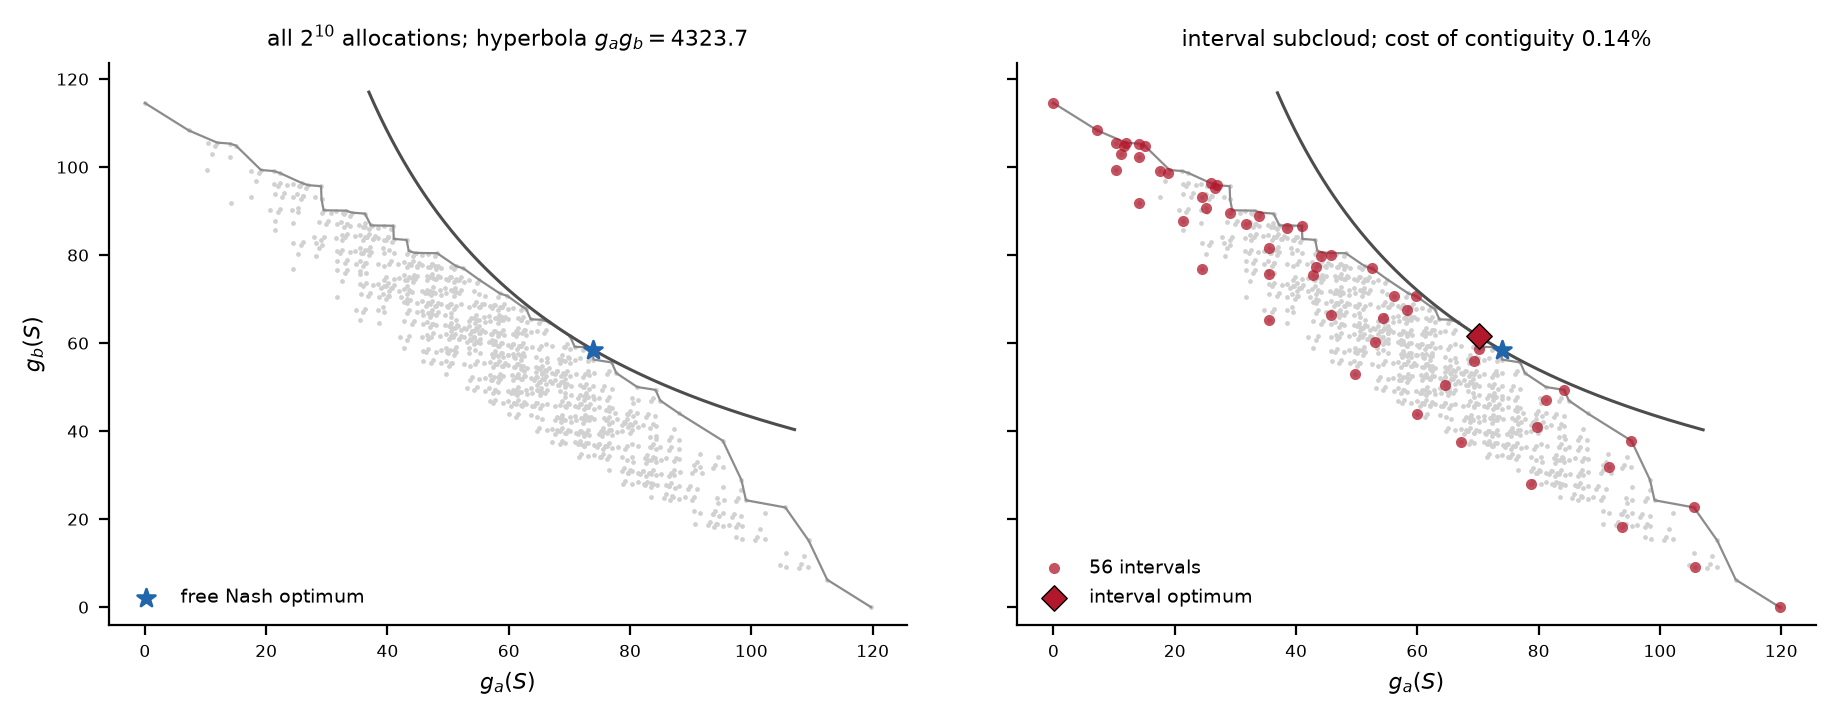
\includegraphics[width=\textwidth]{toy_path.png}
\caption{The path toy. \emph{Left:} all $2^{\pathN}=\pathSubsets$ allocations in gain
space; the grey line is the Pareto frontier, the star the free Nash optimum
$S^\ast=\pathFreeSet$ with $\ga\gb=\pathFreeProd$, and the curve its hyperbola.
\emph{Right:} the \pathIntervals{} allocations in which side $a$'s territory is an
interval (red), their optimum $\pathIvSet$ (diamond), and its lower tangent hyperbola.
The cloud thins, the frontier retreats, the tangency slides.}
\label{fig:path}
\end{figure}

The free optimum is $S^\ast=\pathFreeSet$: \emph{not} an interval --- it skips zip~5
and takes zip~6, because at these draws $\ua(6)/\ub(6)$ beats $\ua(5)/\ub(5)$ and the
tangency prefers the exchange. Requiring side $a$ to be connected restricts the
$\pathSubsets$-point cloud to the $\pathIntervals$ intervals
($\binom{\pathN+1}{2}+1$, verified by the enumeration); the constrained optimum is
$\pathIvSet$ with product \pathIvProd{} against the free \pathFreeProd{} --- a cost of
contiguity of \pathIvCostPct\%. Requiring \emph{both} sides connected is stronger
still on a path (side $a$'s interval must touch an end, else it cuts $b$ in two):
only \pathBothConn{} allocations survive, and here the optimum happens to be the same
prefix $\pathBothSet$, so the extra restriction costs nothing --- an instance of a
general pattern, that most of the cost is paid at the first connectivity requirement.

Both panels of Figure~\ref{fig:path} repay staring. The frontier's near-linearity is
why weighted-sum scalarisation collapses (Section~\ref{sec:geometry}); the vertical gap
between the two hyperbolas \emph{is} the cost of contiguity; and the interval subcloud
hugs the free frontier closely --- at production sizes the measured cost is a few
tenths of a percent, and the toy shows why: connected near-optima crowd the tangency.

\subsection{Sixteen zips on a grid: disconnection and one cut}\label{sec:toygrid}

The path cannot show the failure mode that matters, because on a path the free optimum
rarely fragments badly. Take a $4\times4$ Rook grid (seed \gridSeed) with a
\emph{bimodal} profile for firm A --- two high-$A$ pockets in opposite corners --- and
a high-$B$ band on the anti-diagonal between them. This abstracts failure mechanism
\emph{(a)} of the programme: the free optimum wants both pockets and drops the glue.

\begin{figure}[t]
\centering
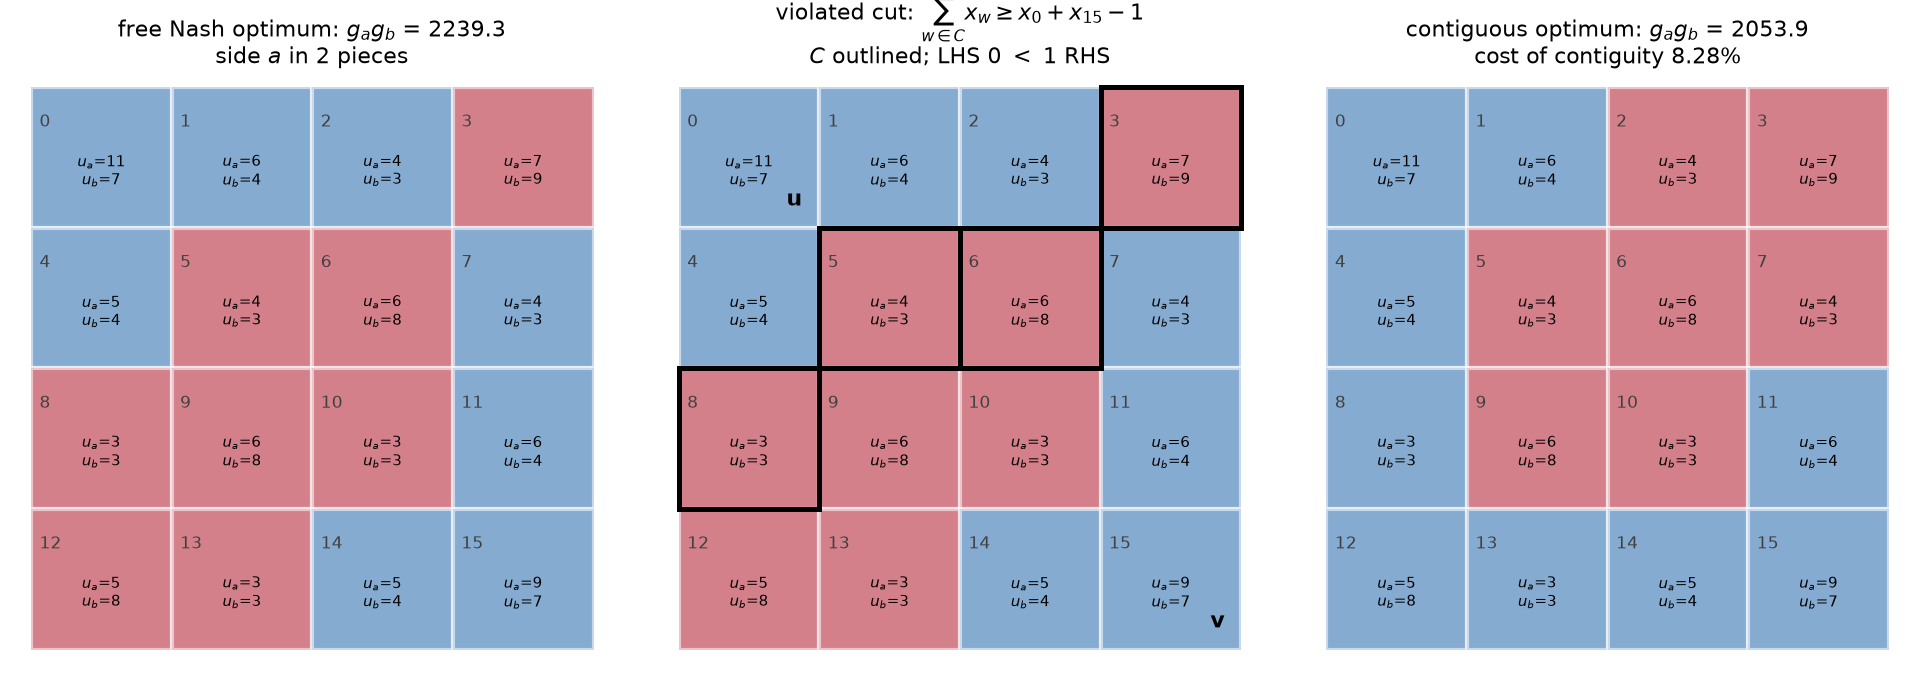
\includegraphics[width=\textwidth]{toy_grid.png}
\caption{The grid toy (side $a$ blue, side $b$ red; per-cell utilities printed).
\emph{Left:} the free Nash optimum puts side $a$'s territory in \gridFreePieces{}
pieces. \emph{Middle:} the root-free separator cut \eqref{eq:sepcut} generated at that
point: $P=\gridPieceP$, endpoints $u=\gridCutU$, $v=\gridCutV$, separator
$C=\gridCutC$ (outlined); the free point has $\sum_{w\in C}x_w=\gridCutLhsFree <
\gridCutRhsFree = x_{\gridCutU}+x_{\gridCutV}-1$. \emph{Right:} the contiguous
optimum buys connectivity through the band.}
\label{fig:grid}
\end{figure}

The free optimum ($\ga\gb=\gridFreeProd$) gives $a$ the set $\gridFreeASet$ ---
\gridFreePieces{} pieces, one per pocket. Of the $2^{16}=\gridSubsets$ allocations only
\gridFeasible{} have both sides connected; the best of them
($\gridContASet$, $\ga\gb=\gridContProd$) keeps one pocket, crosses the band at its
cheapest cell, and reaches the far pocket along the edge --- at a cost of
\gridCostPct\%, an order of magnitude above the path toy's, because here contiguity
binds against the value structure rather than against noise. (The toy is engineered to
make the cost visible; measured production costs sit near $0.4\%$.)

The middle panel shows the solver's actual move at the free point. The smaller piece is
$P=\gridPieceP$; the highest-utility vertices give $u=\gridCutU$, $v=\gridCutV$; the
neighbourhood of $P$, greedily minimalised, gives the separator $C=\gridCutC$. The free
point violates \eqref{eq:sepcut} ($\gridCutLhsFree<\gridCutRhsFree$), the contiguous
optimum satisfies it, and --- the point of the root-free form --- the inequality says
nothing about \emph{where} side $a$ must live, only that it cannot occupy both $u$ and
$v$ without paying for a crossing of $C$. Branch-and-cut adds such inequalities lazily,
each one deleting a slab of the disconnected cloud, until the surviving relaxation's
bound meets an incumbent like the right panel.

\subsection*{What the toys do not show}

Honesty about the abstraction: (i) at $n\le16$ the certificates are instant --- the
dual-bound crawl of Section~\ref{sec:solver} needs hundreds of zips and value
concentration to appear; (ii) real pair graphs arrive already disconnected (islands),
which is what forces the component-wise statement of the constraint and the root-free
cut form; (iii) real instances carry hundreds of near-zero ``glue'' zips whose only
role is connectivity, a regime the reduction layer targets and no 16-cell toy can
imitate.

\bibliographystyle{plainnat}
\bibliography{../../../literature/territory_bibliography}

\end{document}
